\documentclass[10pt,a4paper,twoside]{article}

% \usepackage[margin=2cm]{geometry}
\usepackage[inner=2.5cm,outer=1.5cm,top=1.5cm,bottom=1.5cm]{geometry}
\usepackage{fontspec}
\usepackage[none]{hyphenat}
\setmainfont{Comic Sans MS}
\usepackage[dvipsnames]{xcolor}
\usepackage{graphicx}
\usepackage{tikz}
\usetikzlibrary{shapes.callouts,positioning}
\usepackage[pages=some,placement=top]{background}

\newcommand{\englang}[1]{
    #1 %comment/uncomment this line to hide/show english
}
\newcommand{\italang}[1]{
    % #1 %comment/uncomment this line to hide/show italian
}

% \renewcommand*\familydefault{\sfdefault}

% \pagenumbering{gobble}
\graphicspath{{./figures/}}



\begin{document}

~
\backgroundsetup{
scale=1.1,
angle=0,
opacity=1,  %% adjust
contents={
\includegraphics[keepaspectratio]{cover}}
}
\BgThispage
\thispagestyle{empty}

\newpage
~
\newpage



%%%%%%%%%% PAGE 1
\noindent
\begin{minipage}{1.4\textwidth}
    \begin{tikzpicture}
        \node (img) {\frame{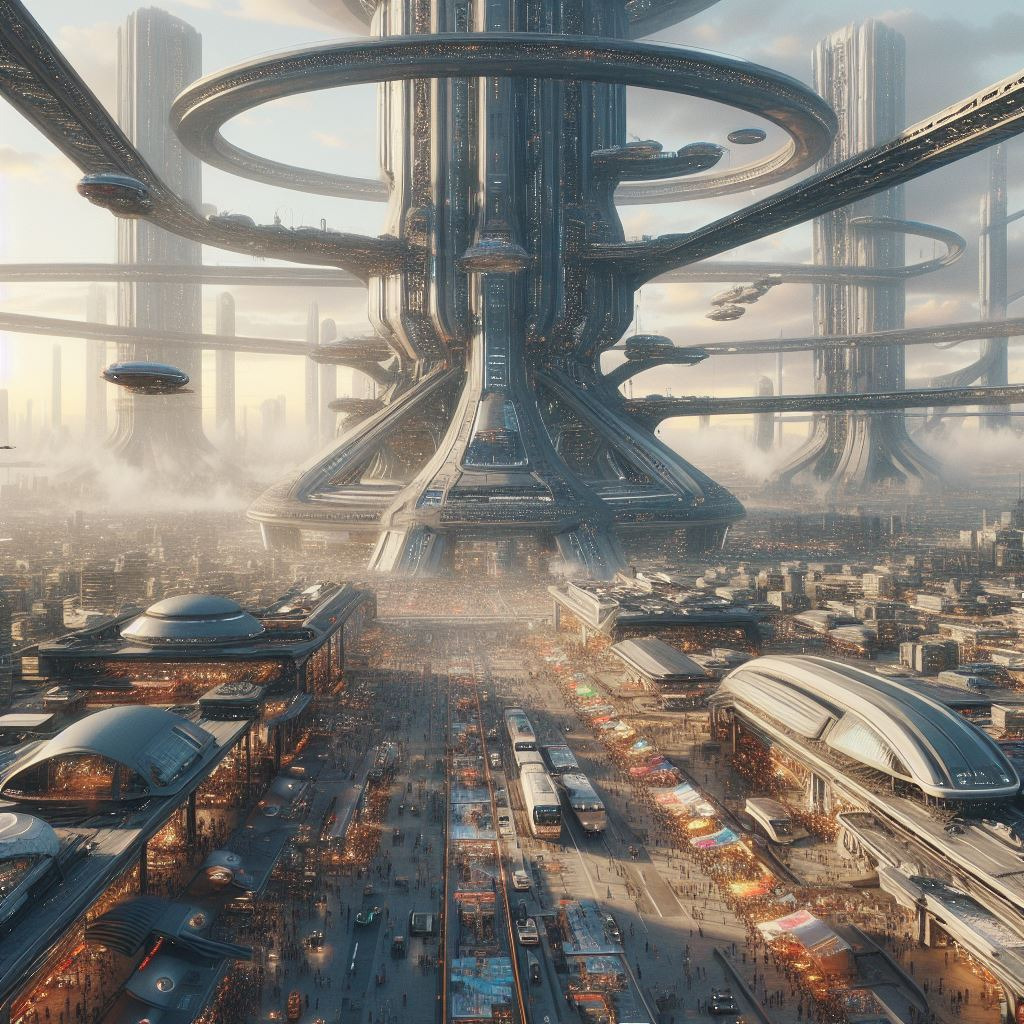
\includegraphics[width=\textwidth]{p1s1}}};
        \node [text width=5cm, align=center, rectangle callout, fill=white, draw, callout relative pointer={(0,0)}] at (-8,10) {
            \englang{SANCTUM PRIME: A HEAVEN BEYOND EARTH}
            \italang{SANCTUM PRIME:\\UN PARADISO OLTRE LA TERRA}
            };
        \node [text width=7cm, align=center, rectangle callout, fill=white, draw, callout relative pointer={(0,0)}] at (2.5,6) {
            \englang{AN ARCOLOGY, LIKE SANCTUM PRIME, STANDS AS A SELF-SUSTAINING OASIS BEYOND EARTH---A TOWERING CITYSCAPE WHERE HUMANITY THRIVES AMIDST THE EXPANSE OF DEEP SPACE, A TESTAMENT TO HUMAN RESILIENCE AND INNOVATION}
            \italang{UN'ARCOLOGIA, COME SANCTUM PRIME, SI ERGE COME UN'OASI AUTOSUFFICIENTE AL DI LÀ DELLA TERRA---UN PAESAGGIO URBANO VERTIGINOSO DOVE L'UMANITÀ PROSPERA NELL'IMMENSITÀ DELLO SPAZIO PROFONDO, UNA TESTIMONIANZA DELLA RESILIENZA E DELL'INNOVAZIONE UMANA}
            };
        \node [text width=6.5cm, align=center, rectangle callout, fill=white, draw, callout relative pointer={(0,0)}] at (-6.5,-7.5) {
            \englang{ARCOLOGIES ARE VERTICAL CITIES, WHERE PEOPLE LIVE, WORK, AND CREATE WITHIN TOWERING STRUCTURES, A MICROCOSM OF CIVILIZATION SUSTAINED BY ADVANCED TECHNOLOGY, PROVIDING SHELTER, RESOURCES, AND COMMUNITY IN THE VASTNESS OF SPACE}
            \italang{LE ARCOLOGIE SONO CITTÀ VERTICALI, DOVE LE PERSONE VIVONO, LAVORANO, E CREANO ALL'INTERNO DI STRUTTURE IMPONENTI, UN MICROCOSMO DI CIVILTÀ SOSTENUTO DA TECNOLOGIE AVANZATE, CHE FORNISCONO RIPARO, RISORSE E COMUNITÀ NELLA VASTITÀ DELLO SPAZIO}
            };
    \end{tikzpicture}
\end{minipage}%

\newpage



%%%%%%%%%% PAGE 2
\noindent
\begin{minipage}{0.49\textwidth}
    \begin{tikzpicture}
        \node (img) {\frame{
\includegraphics[width=\textwidth]{p2s1}}};
        \node [text width=5cm, align=center, rectangle callout, fill=white, draw, callout relative pointer={(0,0)}] at (-1,4) {
            \englang{DR.~EVELYN HAYES, COMMUNICATION SCIENTIST}
            \italang{DOTT.SSA EVELYN HAYES, SCIENZIATA DELLA COMUNICAZIONE}
            };
        \node [text width=2.5cm, align=center, ellipse callout, fill=white, draw, callout relative pointer={(0.5,0.5)}] at (-2,-2.5) {
            \englang{THE SIGNAL PATTERNS ARE PERSISTENT, LILY}
            \italang{I MODELLI DI SEGNALE SONO PERSISTENTI, LILY.}
            };
        \node [text width=2.5cm, align=center, ellipse callout, fill=white, draw, callout relative pointer={(-0.5,1)}] at (2,-3.2) {
            \englang{WHAT DO YOU SEE UP THERE, LILY?}
            \italang{COSA VEDI LASSU, LILY?}
            };
    \end{tikzpicture}
\end{minipage}%
\hfill
\begin{minipage}{0.49\textwidth}
    \begin{tikzpicture}
        \node (img) {\frame{
\includegraphics[width=\textwidth]{p2s2}}};
    \end{tikzpicture}
\end{minipage}%
\vspace{.1cm}
\noindent\hspace{1pt}
\begin{minipage}{1\textwidth}
    \begin{tikzpicture}
        \node (img) {\frame{
\includegraphics[width=\textwidth]{p2s3}}};
        \node [dashed, text width=3cm, align=center, ellipse callout, fill=white, draw, callout relative pointer={(0,0)}] at (5,5) {
            \englang{THEY WANT US TO HEAR THEM.}
            \italang{VOGLIONO CHE LI ASCOLTIAMO.}
            };
        \draw [dashed, fill=white, draw] (4.5,3.5) ellipse (.5cm and .25cm);
        \draw [dashed, fill=white, draw] (3.8,2.8) ellipse (.25cm and .125cm);
    \end{tikzpicture}
\end{minipage}%

\newpage



%%%%%%%%%% PAGE 3
~\vspace{2cm}

\noindent
\begin{minipage}{0.49\textwidth}
    \begin{tikzpicture}
        \node (img) {\frame{
\includegraphics[width=\textwidth]{p3s1}}};
        \node [text width=4.5cm, align=center, ellipse callout, fill=white, draw, callout relative pointer={(0,0.5)}] at (-.5,-3) {
            \englang{THE SIGNAL PATTERNS ARE PERSISTENT, BUT THEIR ORIGIN REMAINS ELUSIVE...}
            \italang{GLI SCHEMI DEL SEGNALE SONO PERSISTENTI, MA LA LORO ORIGINE SEMBRA SFUGGENTE...}
            };
    \end{tikzpicture}
\end{minipage}%
\hfill
\begin{minipage}{0.49\textwidth}
    \begin{tikzpicture}
        \node (img) {\frame{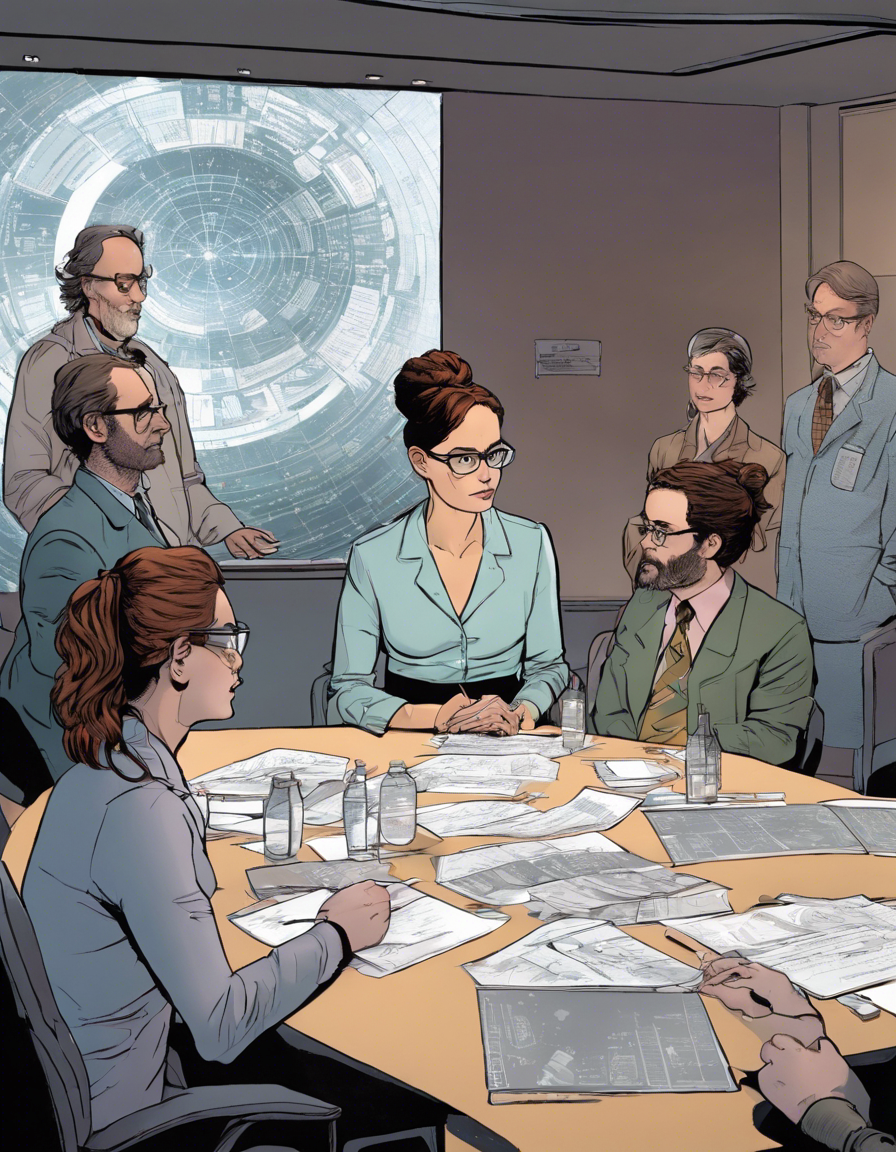
\includegraphics[width=\textwidth]{p3s2}}};
        \node [text width=4.5cm, align=center, ellipse callout, fill=white, draw, callout relative pointer={(-0.5,1.2)}] at (0,-3) {
            \englang{OUR SITUATION IS CRITICAL. WE MUST FIND SOLUTIONS BEFORE IT'S TOO LATE!}
            \italang{
                LA NOSTRA SITUAZIONE È CRITICA. DOBBIAMO TROVARE DELLE SOLUZIONI PRIMA CHE SIA TROPPO TARDI!}
            };
        \node [text width=3.5cm, align=center, rectangle callout, fill=white, draw, callout relative pointer={(0,0)}] at (1.8,3.2) {
            \englang{IN THE MEETING ROOM}
            \italang{NELLA SALA CONFERENZE}
            };
    \end{tikzpicture}
\end{minipage}%
\vspace{2cm}
\noindent\hspace{1pt}
\begin{minipage}{0.49\textwidth}
    \vspace{0.85cm}
    \begin{tikzpicture}
        \node (img) {\frame{
\includegraphics[width=\textwidth]{p3s3}}};
        \node [text width=3.5cm, align=center, rectangle callout, fill=white, draw, callout relative pointer={(0,0)}] at (-1.8,3.2) {
            \englang{BACK IN THE QUARTERS}
            \italang{NEGLI ALLOGGI}
            };
        \node [dashed, text width=2.5cm, align=center, ellipse callout, fill=white, draw, callout relative pointer={(0,0)}] at (-2,-3.5) {
            \englang{THEY'RE ASKING FOR HELP. I CAN FEEL IT.}
            \italang{STANNO CHIEDENDO AIUTO. LO SENTO.}
            };
        \draw [dashed, fill=white, draw] (-2.2,-1.1) ellipse (.5cm and .25cm);
        \draw [dashed, fill=white, draw] (-1.8,-0.6) ellipse (.25cm and .125cm);
    \end{tikzpicture}
\end{minipage}%
\hfill
\begin{minipage}{0.49\textwidth}
    \begin{tikzpicture}
        \node (img) {\frame{
\includegraphics[width=\textwidth]{p3s4}}};
        \node [text width=2.5cm, align=center, ellipse callout, fill=white, draw, callout relative pointer={(-0.5,-0.5)}] at (2,3) {
            \englang{LILY, YOU SHOULDN'T BE SEEING THIS. IT'S NOT SAFE.}
            \italang{LILY, NON DOVRESTI VEDERE TUTTO QUESTO. NON È SICURO.}
            };
    \end{tikzpicture}
\end{minipage}%

\newpage



%%%%%%%%%% PAGE 4
~\vspace{2cm}

\noindent
\begin{minipage}{0.49\textwidth}
    \begin{tikzpicture}
        \node (img) {\frame{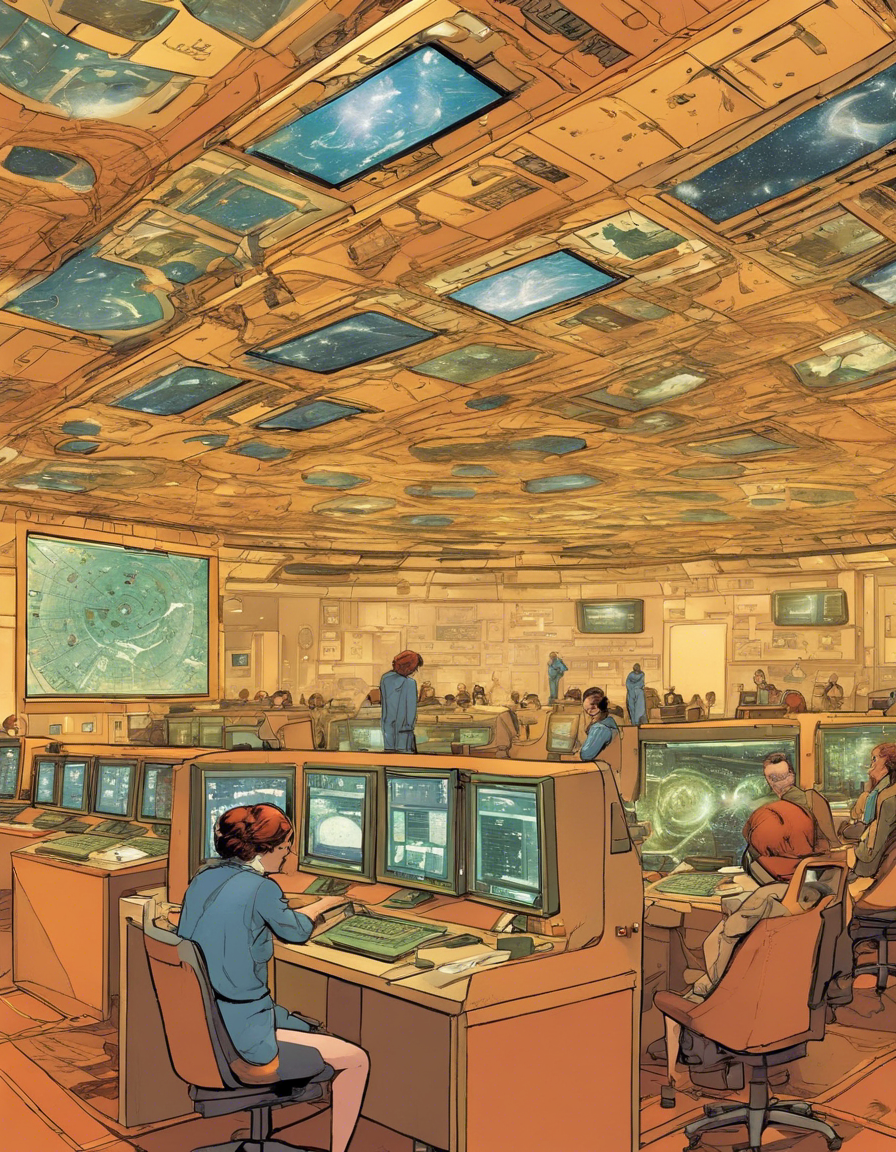
\includegraphics[width=\textwidth]{p4s1}}};
        \node [text width=3.5cm, align=center, rectangle callout, fill=white, draw, callout relative pointer={(0,0)}] at (-1.8,3.2) {
            \englang{IN THE COMMUNICATION STATION}
            \italang{NELLA STAZIONE DI COMUNICAZIONE}
            };
        \node [text width=4.5cm, align=center, ellipse callout, fill=white, draw, callout relative pointer={(0,-1)}] at (0.5,1.2) {
            \englang{WHAT'S HAPPENING? THIS IS UNPRECEDENTED!}
            \italang{COSA STA SUCCEDENDO? È SENZA PRECEDENTI!}
            };
    \end{tikzpicture}
\end{minipage}%
\hfill
\begin{minipage}{0.49\textwidth}
    \vspace{0.45cm}
    \begin{tikzpicture}
        \node (img) {\frame{
\includegraphics[width=\textwidth]{p4s2}}};
        \node [text width=4cm, align=center, ellipse callout, fill=white, draw, callout relative pointer={(0.5,1)}] at (-1,-4) {
            \englang{THIS SIGNAL---IT'S A CRY FOR HELP!}
            \italang{QUESTO SEGNALE---È UN GRIDO D'AIUTO!}
            };
    \end{tikzpicture}
\end{minipage}%
\vspace{1.2cm}
\noindent\hspace{1pt}
\begin{minipage}{0.49\textwidth}
    \begin{tikzpicture}
        \node (img) {\frame{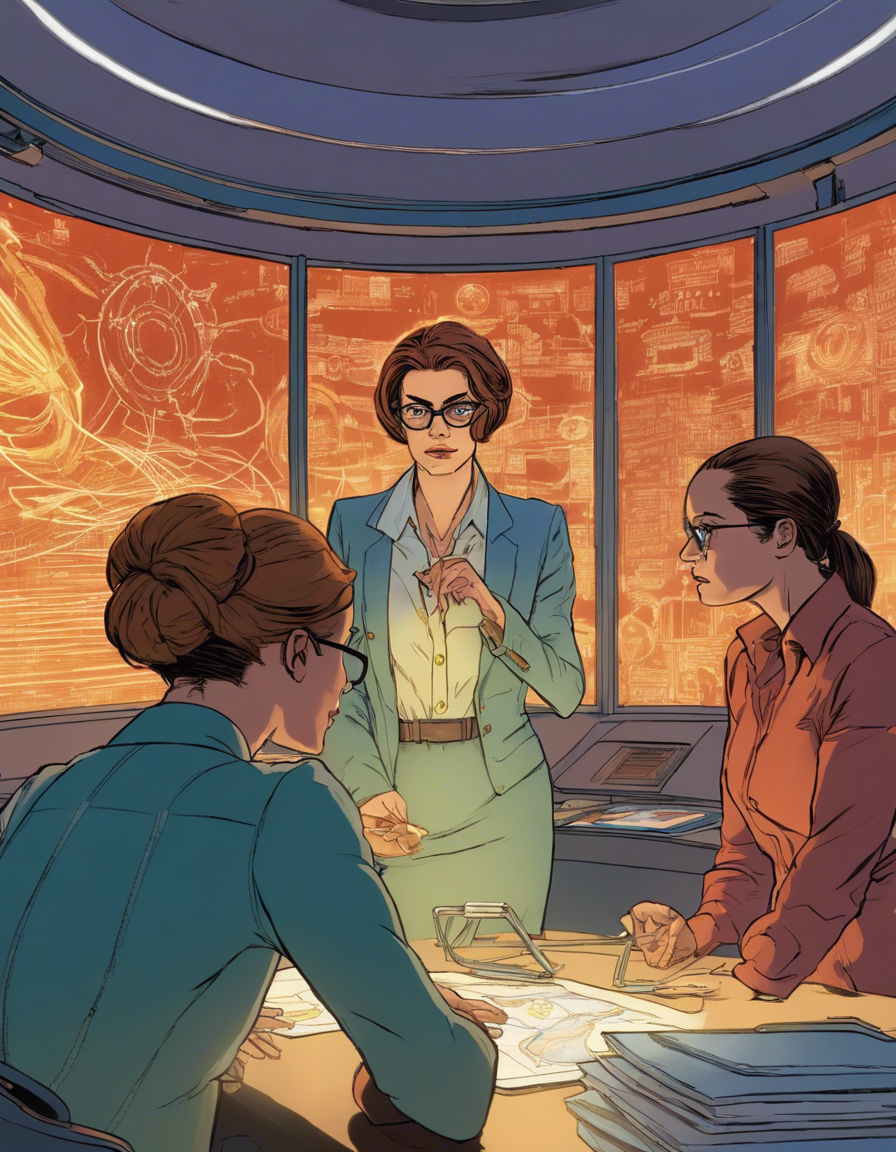
\includegraphics[width=\textwidth]{p4s3}}};
        \node [text width=3cm, align=center, ellipse callout, fill=white, draw, callout relative pointer={(0.2,-0.5)}] at (-1.8,3.5) {
            \englang{WE NEED TO ACT FAST! LIVES MAY BE AT STAKE!}
            \italang{DOBBIAMO AGIRE VELOCEMENTE! DELLE VITE POTREBBERO ESSERE IN PERICOLO!}
            };
    \end{tikzpicture}
\end{minipage}%
\hfill
\begin{minipage}{0.49\textwidth}
    \vspace{2.05cm}
    \begin{tikzpicture}
        \node (img) {\frame{
\includegraphics[width=\textwidth]{p4s4}}};
        \node [text width=5cm, align=center, ellipse callout, fill=white, draw, callout relative pointer={(0,1)}] at (0,-4.2) {
            \englang{PREPARE THE EXPEDITION. WE'RE GOING TO INVESTIGATE THE SOURCE OF THIS SIGNAL OURSELVES.}
            \italang{PREPARATE L'ESPLORAZIONE. È ORA DI INDAGARE SULLA FONTE DI QUESTO SEGNALE.}
            };
    \end{tikzpicture}
\end{minipage}%

\newpage 



%%%%%%%%%% PAGE 5
~\vspace{2.5cm}

\noindent
\begin{minipage}{0.49\textwidth}
    \begin{tikzpicture}
        \node (img) {\frame{
\includegraphics[width=\textwidth]{p5s1}}};
        \node [text width=2cm, align=center, ellipse callout, fill=white, draw, callout relative pointer={(0,-1)}] at (2.5,1.2) {
            \englang{THEY'RE SCARED. I CAN FEEL IT.}
            \italang{HANNO PAURA. LO SENTO.}
            };
    \end{tikzpicture}
\end{minipage}%
\hfill
\begin{minipage}{0.49\textwidth}
    \begin{tikzpicture}
        \node (img) {\frame{
\includegraphics[width=\textwidth]{p5s2}}};
        \node [text width=2.5cm, align=center, ellipse callout, fill=white, draw, callout relative pointer={(0,0.5)}] at (-2,-2.5) {
            \englang{LILY, YOU SHOULDN'T BE SEEING THIS. IT'S NOT SAFE.}
            \italang{LILY, NON DOVRESTI VEDERE TUTTO QUESTO. NON È SICURO.}
            };
    \end{tikzpicture}
\end{minipage}%
\vspace{2.3cm}
\noindent\hspace{1pt}
\begin{minipage}{0.49\textwidth}
    \vspace{0.4cm}
    \begin{tikzpicture}
        \node (img) {\frame{
\includegraphics[width=\textwidth]{p5s3}}};
        \node [text width=2.4cm, align=center, ellipse callout, fill=white, draw, callout relative pointer={(0.5,0)}] at (-2.2,0.5) {
            \englang{THEY'RE ASKING FOR HELP. WE HAVE TO DO SOMETHING.}
            \italang{STANNO CHIEDENDO AIUTO. DOBBIAMO FARE QUALCOSA.}
            };
    \end{tikzpicture}
\end{minipage}%
\hfill
\begin{minipage}{0.49\textwidth}
    \begin{tikzpicture}
        \node (img) {\frame{
\includegraphics[width=\textwidth]{p5s4}}};
        \node [dashed, text width=2.5cm, align=center, ellipse callout, fill=white, draw, callout relative pointer={(0,0)}] at (-2.2,2.2) {
            \englang{PERHAPS LILY HOLDS THE KEY TO UNLOCKING THE MYSTERY BEHIND THIS SIGNAL.}
            \italang{FORSE LILY È LA CHIAVE PER SCOPRIRE IL MISTERO DI QUESTO SEGNALE.}
            };
        \draw [dashed, fill=white, draw] (-0.2,4) ellipse (.5cm and .25cm);
        \draw [dashed, fill=white, draw] (0.3,3.5) ellipse (.25cm and .125cm);
    \end{tikzpicture}
\end{minipage}%

\newpage 



%%%%%%%%%% PAGE 6
~\vspace{2cm}

\noindent
\begin{minipage}{0.49\textwidth}
    \vspace{0.8cm}
    \begin{tikzpicture}
        \node (img) {\frame{
\includegraphics[width=\textwidth]{p6s1}}};
        \node [dashed, text width=3cm, align=center, ellipse callout, fill=white, draw, callout relative pointer={(0,0)}] at (-1.5,-3) {
            \englang{HOW DOES SHE UNDERSTAND?}
            \italang{COME FA A CAPIRE?}
            };
        \draw [dashed, fill=white, draw] (-2.2,-1.6) ellipse (.5cm and .25cm);
        \draw [dashed, fill=white, draw] (-2,-0.8) ellipse (.25cm and .125cm);
    \end{tikzpicture}
\end{minipage}%
\hfill
\begin{minipage}{0.49\textwidth}
    \begin{tikzpicture}
        \node (img) {\frame{
\includegraphics[width=\textwidth]{p6s2}}};
        \node [text width=2.7cm, align=center, ellipse callout, fill=white, draw, callout relative pointer={(-0.3,-0.5)}] at (2,3.5) {
            \englang{WE NEED TO UNITE OUR EXPERTISE. OUR MISSION IS CLEAR.}
            \italang{DOBBIAMO UNIRE LE NOSTRE COMPETENZE. LA NOSTRA MISSIONE È CHIARA.}
            };
    \end{tikzpicture}
\end{minipage}%
\vspace{2.4cm}
\noindent\hspace{1pt}
\begin{minipage}{0.49\textwidth}
    \vspace{0.25cm}
    \begin{tikzpicture}
        \node (img) {\frame{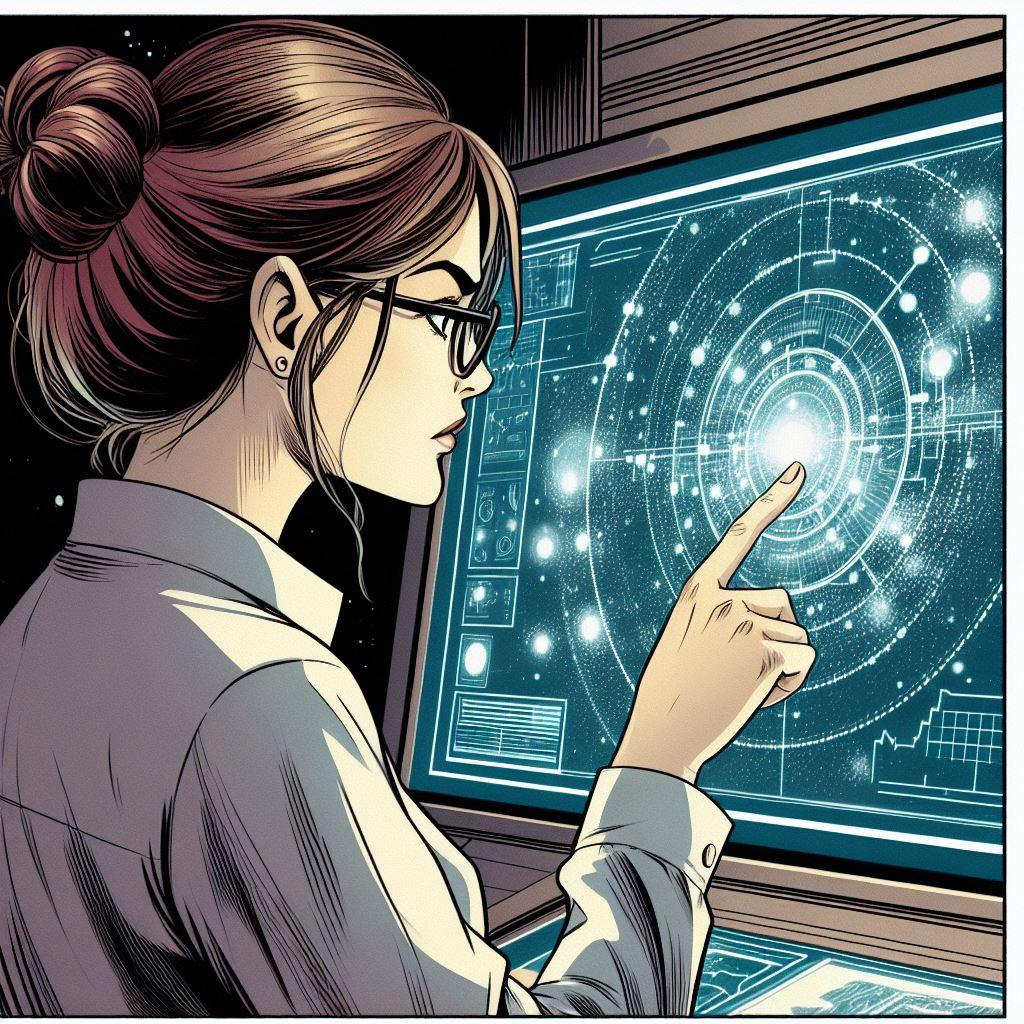
\includegraphics[width=\textwidth]{p6s3}}};
        \node [text width=4cm, align=center, ellipse callout, fill=white, draw, callout relative pointer={(0,0.5)}] at (-1,-3.5) {
            \englang{OUR DESTINATION LIES BEYOND THE ARCOLOGY'S REACH. BUT WE MUST GO WHERE THE SIGNAL LEADS US.}
            \italang{LA NOSTRA DESTINAZIONE È AL DI LÀ DELLA PORTATA DELL'ARCOLOGIA. MA DOBBIAMO ANDARE DOVE CI PORTA IL SEGNALE.}
            };
    \end{tikzpicture}
\end{minipage}%
\hfill
\begin{minipage}{0.49\textwidth}
    \begin{tikzpicture}
        \node (img) {\frame{
\includegraphics[width=\textwidth]{p6s4}}};
        \node [text width=5cm, align=center, ellipse callout, fill=white, draw, callout relative pointer={(0,0.5)}] at (0,-4.2) {
            \englang{WE CANNOT IGNORE THEIR CALL. OUR JOURNEY BEGINS NOW.}
            \italang{NON POSSIAMO IGNORARE IL LORO APPELLO. IL NOSTRO VIAGGIO INIZIA ORA.}
            };
    \end{tikzpicture}
\end{minipage}%

\newpage 



%%%%%%%%%% PAGE 7
% ~\vspace{2cm}

\noindent
\begin{minipage}{0.75\textwidth}
    \hspace{1.37cm}
    \begin{tikzpicture}
        \node (img) {\frame{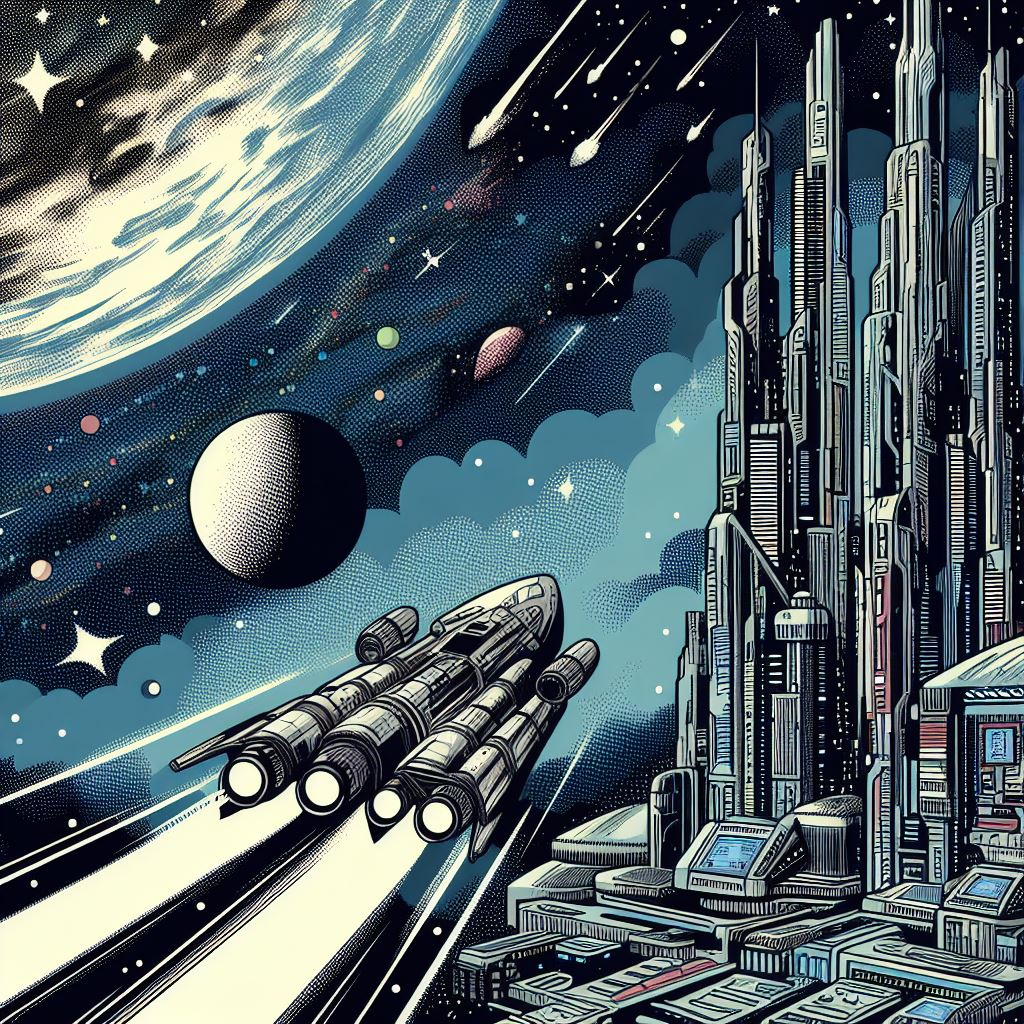
\includegraphics[width=\textwidth]{p7s1}}};
        \node [text width=5cm, align=center, rectangle callout, fill=white, draw, callout relative pointer={(0,0)}] at (-4.5,3.5) {
            \englang{WE'RE HEADING INTO THE UNKNOWN. BUT WE MUST GO WHERE THE SIGNAL LEADS US.}
            \italang{CI STIAMO INOLTRANDO NELL'IGNOTO. MA DOBBIAMO ANDARE DOVE CI PORTA IL SEGNALE.}
            };
    \end{tikzpicture}
\end{minipage}%

\vspace{0.2cm}

\noindent%\hspace{1pt}
\begin{minipage}{0.75\textwidth}
    \hspace{2cm}
    \begin{tikzpicture}
        \node (img) {\frame{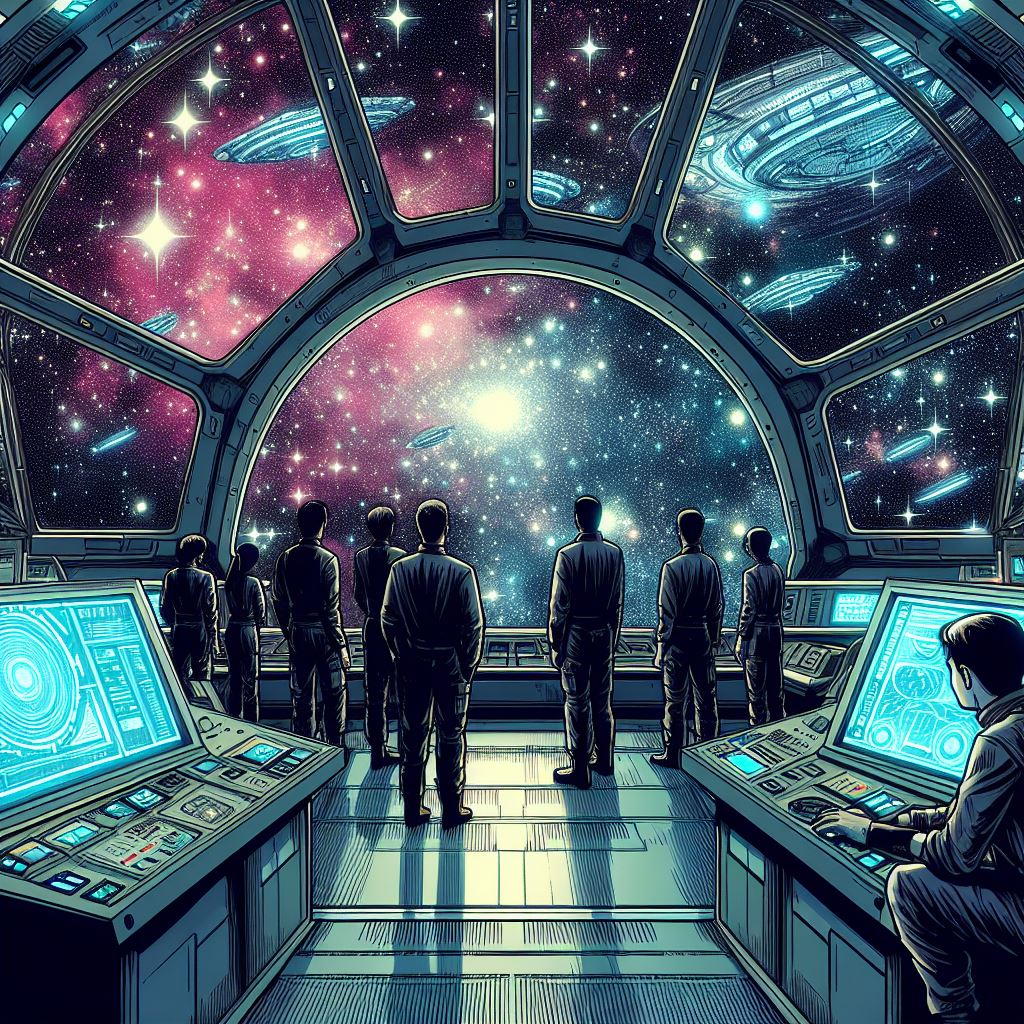
\includegraphics[width=\textwidth]{p7s2}}};
        \node [text width=5cm, align=center, ellipse callout, fill=white, draw, callout relative pointer={(-1,-0.5)}] at (4.5,2.5) {
            \englang{THIS IS BEYOND ANYTHING WE IMAGINED! BUT WE'RE READY FOR WHATEVER LIES AHEAD.}
            \italang{QUESTO È AL DI LÀ DI QUALSIASI COSA AVESSIMO IMMAGINATO! MA SIAMO PRONTI PER QUALSIASI COSA CI ASPETTI.}
            };
    \end{tikzpicture}
\end{minipage}%

\newpage 



\end{document}